% !TeX root = ./thesis.tex










%==============================
\cleardoublepage
\thispagestyle{empty}

\vspace*{55pt}

\begin{centering}
	{\fontspec[Ligatures={Common,Rare,Historic,TeX}, Numbers={OldStyle}, AutoFakeBold=1.5]{Anaktoria}
		{
		\setbox0=\hbox{{Proof is boring. Proof is tiresome. Proof is an irrelevance.}}
		\setbox1=\hbox{\Large``}
		\begin{minipage}{\wd0}
			\raisebox{-.5ex}{\hspace*{-.65\wd1}{\color{P1797}\Large ``\normalcolor}\hspace*{-.35\wd1}}%
				{Proof is boring\color{P1797}\textbf{.}\normalcolor\ Proof is tiresome\color{P1797}\textbf{.}\normalcolor\ Proof is an irrelevance\color{P1797}\textbf{.}\normalcolor\\
				People would far rather be handed an easy lie\\
				than search for a difficult truth\color{P1797}\textbf{,}\normalcolor\\
				especially if it suits their own purposes\color{P1797}\textbf{.}\normalcolor}%
			\raisebox{-.75ex}{\hspace*{-.45\wd1}{\color{P1797}\Large ''\normalcolor}\hspace*{-.35\wd1}}%
			\\
			\normalcolor\normalfont\normalsize\null \hfill---Joe Abercrombie, \emph{Last Argument of Kings}, 2008.
		\end{minipage}}
		\par}
\end{centering}


%==============================
\cleardoublepage
\thispagestyle{empty}

\null\vfill
\noindent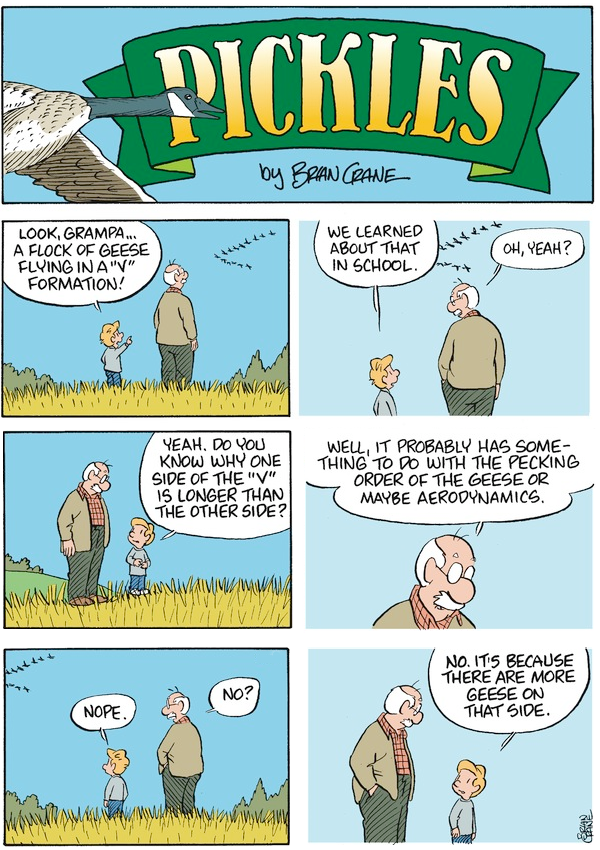
\includegraphics[width=\textwidth]{pickles2}
\vfill

